
\subsection{Answers}
\begin{table}[htb]%
\begin{center}%
\caption{Q19: What are your obstacles to mastering MPI?}%
\label{tab:Q19-ans}%
\begin{tabular}{l|l|r}%
\hline%
Choice & Abbrv. & \# Answers \\%
\hline%
I have no obstacles. & No obstacles & 332 (41.3\%) \\%
Too many routines. & Too many routines & 169 (21.0\%) \\%
Too complicated and hard to understand. & Complicated & 115 (14.3\%) \\%
No appropriate lecture / book / info. & No appropriate one & 110 (13.7\%) \\%
I have nobody to ask. & Nobody to ask & 83 (10.3\%) \\%
I do not like the API. & Dislike API & 68 (8.5\%) \\%
other & - & 111 (13.8\%) \\%
\hline%
\multicolumn{2}{c}{total} & 988 (803)\\%
\hline%
\end{tabular}%
\end{center}%
\end{table}%

\clearpage%
{\footnotesize\begin{landscape}%
\begin{longtable}[htb]{r|c|c|c|c|c|c|c|c|c|c}%
\caption{Q19: What are your obstacles to mastering MPI?}%
\label{tab:Q19-mans} \\%
\hline%
Multi-Answer & overall & FR & GR & IT & UK & eu & JP & RU & US & others \\
 \hline%
\endfirsthead%
\multicolumn{11}{r}{(continued from the previous page)}\\%
\hline%
Multi-Answer & overall & FR & GR & IT & UK & eu & JP & RU & US & others \\
 \hline%
\endhead%
\hline%
(total) & 803 & 118 & 149 & 54 & 62 & 131 & 63 & 92 & 54 & 80 \\%
\hline%
\multicolumn{11}{r}{(continue to the next page)}\\%
\endfoot%
\hline%
(total) & 803 & 118 & 149 & 54 & 62 & 131 & 63 & 92 & 54 & 80 \\%
\hline%
\endlastfoot%
\hline%
{No obstacles} & 302 & 48 & 56 & 20 & 19 & 55 & 19 & 40 & 24 & 21 \\%
{Too many routines} & 93 & 15 & 19 & 8 & 4 & 14 & 13 & 8 & 6 & 6 \\%
{No appropriate one} & 56 & 8 & 6 & 3 & 2 & 12 & 7 & 8 & 1 & 9 \\%
{Nobody to ask} & 47 & 2 & 12 & 4 & 6 & 5 & 0 & 11 & 3 & 4 \\%
{Complicated} & 46 & 6 & 7 & 3 & 4 & 4 & 6 & 5 & 0 & 11 \\%
{Dislike API} & 26 & 3 & 6 & 2 & 1 & 7 & 2 & 1 & 2 & 2 \\%
{Too many routines, No appropriate one} & 16 & 2 & 0 & 1 & 0 & 2 & 4 & 0 & 3 & 4 \\%
{No obstacles, Too many routines} & 16 & 1 & 2 & 1 & 7 & 1 & 1 & 2 & 0 & 1 \\%
{No appropriate one, Nobody to ask} & 15 & 3 & 1 & 2 & 0 & 2 & 0 & 3 & 0 & 4 \\%
{Too many routines, Complicated} & 15 & 1 & 3 & 1 & 3 & 1 & 4 & 0 & 0 & 2 \\%
{Complicated, Nobody to ask} & 10 & 1 & 2 & 0 & 0 & 2 & 1 & 1 & 1 & 2 \\%
{Complicated, Dislike API} & 9 & 3 & 2 & 0 & 0 & 0 & 1 & 2 & 0 & 1 \\%
{Too many routines, Dislike API} & 8 & 0 & 2 & 0 & 0 & 3 & 0 & 0 & 2 & 1 \\%
{No appropriate one, Complicated} & 8 & 0 & 1 & 0 & 0 & 3 & 1 & 0 & 1 & 2 \\%
{Too many routines, Complicated, Dislike API} & 8 & 2 & 2 & 1 & 1 & 0 & 0 & 2 & 0 & 0 \\%
{No appropriate one, Dislike API} & 3 & 0 & 1 & 1 & 0 & 0 & 0 & 0 & 1 & 0 \\%
{No appropriate one, Complicated, Nobody to ask} & 3 & 1 & 0 & 0 & 1 & 0 & 0 & 0 & 0 & 1 \\%
{No obstacles, No appropriate one} & 2 & 1 & 0 & 1 & 0 & 0 & 0 & 0 & 0 & 0 \\%
{Too many routines, No appropriate one, Complicated} & 2 & 0 & 0 & 0 & 0 & 1 & 0 & 0 & 0 & 1 \\%
{No obstacles, Dislike API} & 2 & 1 & 0 & 0 & 0 & 0 & 0 & 1 & 0 & 0 \\%
{Too many routines, Nobody to ask} & 2 & 0 & 0 & 0 & 1 & 1 & 0 & 0 & 0 & 0 \\%
{Open-MPI is routinely buggy and prevents me from using MPI 3.0 as specified} & 2 & 0 & 0 & 0 & 0 & 0 & 0 & 0 & 2 & 0 \\%
{Nobody to ask, Dislike API} & 2 & 0 & 1 & 0 & 1 & 0 & 0 & 0 & 0 & 0 \\%
{Complicated, Dislike API, seems target to Fortran 77 programmers} & 1 & 1 & 0 & 0 & 0 & 0 & 0 & 0 & 0 & 0 \\%
{Too many routines, Complicated, Dislike API, no good Java support} & 1 & 0 & 0 & 0 & 0 & 1 & 0 & 0 & 0 & 0 \\%
{I am at the beginning of learning, so I cannot say yet.} & 1 & 0 & 0 & 0 & 0 & 1 & 0 & 0 & 0 & 0 \\%
{Complicated, Nobody to ask, lack of experience} & 1 & 0 & 0 & 0 & 0 & 1 & 0 & 0 & 0 & 0 \\%
{Incomplete specifications that leave room for interpretation and force me to look into implementation source code therefore worrying me about portability across implementations} & 1 & 0 & 0 & 0 & 0 & 0 & 0 & 0 & 1 & 0 \\%
{Undocumented behavior} & 1 & 0 & 1 & 0 & 0 & 0 & 0 & 0 & 0 & 0 \\%
{performance portable  implentation specific workarounds for bugs} & 1 & 0 & 0 & 0 & 1 & 0 & 0 & 0 & 0 & 0 \\%
{Many implementations.} & 1 & 0 & 0 & 0 & 0 & 0 & 1 & 0 & 0 & 0 \\%
{not my main priority / lack of time} & 1 & 0 & 0 & 0 & 0 & 1 & 0 & 0 & 0 & 0 \\%
{Unexpected running times of MPI routines such as slow MPI\_Comm\_create,...} & 1 & 0 & 1 & 0 & 0 & 0 & 0 & 0 & 0 & 0 \\%
{Too much else to do!} & 1 & 0 & 0 & 0 & 1 & 0 & 0 & 0 & 0 & 0 \\%
{Complicated, Difficult to reason performance numbers.} & 1 & 0 & 0 & 0 & 0 & 0 & 1 & 0 & 0 & 0 \\%
{Difficulty to debug} & 1 & 1 & 0 & 0 & 0 & 0 & 0 & 0 & 0 & 0 \\%
{Limited lectures/tutorials are available online} & 1 & 0 & 0 & 0 & 0 & 0 & 0 & 0 & 0 & 1 \\%
{lack of time} & 1 & 1 & 0 & 0 & 0 & 0 & 0 & 0 & 0 & 0 \\%
{Too many routines, Lack in proper vendor/platform support} & 1 & 0 & 1 & 0 & 0 & 0 & 0 & 0 & 0 & 0 \\%
{Discrepancies between specification and real implementations/implementation quirks, unpredictable interactions between application and MPI implementation behaviour} & 1 & 0 & 0 & 0 & 1 & 0 & 0 & 0 & 0 & 0 \\%
{No detailed and clear enough documents about internal implementation} & 1 & 1 & 0 & 0 & 0 & 0 & 0 & 0 & 0 & 0 \\%
{I know the subset of the standard required to achieve my goals.} & 1 & 0 & 0 & 0 & 1 & 0 & 0 & 0 & 0 & 0 \\%
{difference of implementation and behavior depending on the system. One thing works perfectly on one system and breaks down on another due to vendor tweaks.} & 1 & 1 & 0 & 0 & 0 & 0 & 0 & 0 & 0 & 0 \\%
{I do not develop too many MPI applications, and the ones I maintain do not need too much further parallel optimisation} & 1 & 0 & 0 & 0 & 0 & 1 & 0 & 0 & 0 & 0 \\%
{Time to practice.} & 1 & 0 & 0 & 0 & 0 & 0 & 0 & 0 & 1 & 0 \\%
{No obstacles, renovations of MPI implementation (e.g. VisualStudio), need to adjust environment according to them} & 1 & 0 & 0 & 0 & 0 & 0 & 0 & 1 & 0 & 0 \\%
{Complicated, MPI details are low priority in current tasks, done by colleagues} & 1 & 0 & 1 & 0 & 0 & 0 & 0 & 0 & 0 & 0 \\%
{No obstacles, time} & 1 & 0 & 1 & 0 & 0 & 0 & 0 & 0 & 0 & 0 \\%
{Time limit} & 1 & 0 & 0 & 0 & 0 & 1 & 0 & 0 & 0 & 0 \\%
{No immediate need to do so} & 1 & 0 & 1 & 0 & 0 & 0 & 0 & 0 & 0 & 0 \\%
{Performance/application issues such as appropriate progression} & 1 & 0 & 0 & 0 & 1 & 0 & 0 & 0 & 0 & 0 \\%
{i am supervising a group of developers} & 1 & 0 & 1 & 0 & 0 & 0 & 0 & 0 & 0 & 0 \\%
{Complicated, Light-weight simplified interface. Perhaps OO C++ wrapper.} & 1 & 0 & 0 & 0 & 0 & 1 & 0 & 0 & 0 & 0 \\%
{No obstacles, MPI should allow doing in-place operations by specifying identical pointers for send and receive buffer} & 1 & 0 & 1 & 0 & 0 & 0 & 0 & 0 & 0 & 0 \\%
{No obstacles, It requires time} & 1 & 1 & 0 & 0 & 0 & 0 & 0 & 0 & 0 & 0 \\%
{Too many runtime "optimisation" (implem choice) flags} & 1 & 1 & 0 & 0 & 0 & 0 & 0 & 0 & 0 & 0 \\%
{I do not write any but use them} & 1 & 0 & 0 & 0 & 0 & 1 & 0 & 0 & 0 & 0 \\%
{Complicated, Generally over-engineered IMO} & 1 & 0 & 1 & 0 & 0 & 0 & 0 & 0 & 0 & 0 \\%
{I have no time} & 1 & 1 & 0 & 0 & 0 & 0 & 0 & 0 & 0 & 0 \\%
{No obstacles, The issue is usually the support on supercomputers} & 1 & 1 & 0 & 0 & 0 & 0 & 0 & 0 & 0 & 0 \\%
{confusion between specification of MPI datatypes and standard Fortran types (e.g. the size of MPI Offset kind)} & 1 & 0 & 1 & 0 & 0 & 0 & 0 & 0 & 0 & 0 \\%
{Today I use it only occasionally} & 1 & 1 & 0 & 0 & 0 & 0 & 0 & 0 & 0 & 0 \\%
{Thinking in parallel paradigm} & 1 & 0 & 1 & 0 & 0 & 0 & 0 & 0 & 0 & 0 \\%
{Time} & 1 & 1 & 0 & 0 & 0 & 0 & 0 & 0 & 0 & 0 \\%
{Poor integration with threading libraries, slow adoption to new technologies} & 1 & 0 & 0 & 0 & 0 & 0 & 0 & 0 & 1 & 0 \\%
{Complicated, Dislike API, Difficulty of using outside C/Fortran} & 1 & 0 & 0 & 0 & 0 & 0 & 0 & 0 & 1 & 0 \\%
{Removed C++ interface, exceptions!!!, int32 for most of counts, displ, etc.} & 1 & 0 & 0 & 0 & 0 & 1 & 0 & 0 & 0 & 0 \\%
{Not enough time} & 1 & 0 & 0 & 1 & 0 & 0 & 0 & 0 & 0 & 0 \\%
{Dislike API, type signatures of many prototypes suck (int for sizes, missing const qualifiers, for instance).} & 1 & 1 & 0 & 0 & 0 & 0 & 0 & 0 & 0 & 0 \\%
{Need: I only use it when required for my work.} & 1 & 0 & 0 & 0 & 1 & 0 & 0 & 0 & 0 & 0 \\%
{Nobody to ask, Interfacing with external libraries (e.g. using pnetcdf with MPI is not trivial)} & 1 & 0 & 0 & 1 & 0 & 0 & 0 & 0 & 0 & 0 \\%
{Too many routines, No appropriate one, Complicated, Dislike API} & 1 & 0 & 0 & 0 & 0 & 1 & 0 & 0 & 0 & 0 \\%
{In general carefully understanding all the calls and parameters} & 1 & 0 & 0 & 0 & 0 & 0 & 0 & 0 & 1 & 0 \\%
{Nobody to ask, Time} & 1 & 0 & 0 & 0 & 1 & 0 & 0 & 0 & 0 & 0 \\%
{Have not kept up with recent changes} & 1 & 1 & 0 & 0 & 0 & 0 & 0 & 0 & 0 & 0 \\%
{Lack of time} & 1 & 1 & 0 & 0 & 0 & 0 & 0 & 0 & 0 & 0 \\%
{No exception handling -\verb!>! Inconsisten states} & 1 & 0 & 1 & 0 & 0 & 0 & 0 & 0 & 0 & 0 \\%
{No good and free debuging tools} & 1 & 0 & 0 & 0 & 0 & 0 & 0 & 1 & 0 & 0 \\%
{Other work} & 1 & 0 & 0 & 0 & 0 & 0 & 0 & 0 & 0 & 1 \\%
{Too many routines, Implementations based on the MPI specification depend on vendors.} & 1 & 0 & 0 & 0 & 0 & 0 & 1 & 0 & 0 & 0 \\%
{Too many routines, The practical details of using a certain MPI in a certain way on a certain system makes a lot of other wise simple things hard (debuggers, pinning, start up sanity, terminal IO, file IO, ..)} & 1 & 0 & 0 & 0 & 0 & 1 & 0 & 0 & 0 & 0 \\%
{implementation issues} & 1 & 0 & 1 & 0 & 0 & 0 & 0 & 0 & 0 & 0 \\%
{the message passing paradigm} & 1 & 0 & 0 & 0 & 0 & 0 & 0 & 0 & 0 & 1 \\%
{I don't need to master it} & 1 & 1 & 0 & 0 & 0 & 0 & 0 & 0 & 0 & 0 \\%
{time to spend on it} & 1 & 0 & 0 & 1 & 0 & 0 & 0 & 0 & 0 & 0 \\%
{No obstacles, I have no reason to improve my skills (right now)} & 1 & 0 & 0 & 0 & 0 & 0 & 0 & 1 & 0 & 0 \\%
{GPU programming becomes too complicated} & 1 & 0 & 0 & 0 & 0 & 0 & 0 & 1 & 0 & 0 \\%
{Making sense of the errors that are reported. Often they are not clear about the exact cause, especially when resources are exhausted.} & 1 & 0 & 0 & 0 & 1 & 0 & 0 & 0 & 0 & 0 \\%
{Understanding performance, making immediate communications asynchronous, ...} & 1 & 1 & 0 & 0 & 0 & 0 & 0 & 0 & 0 & 0 \\%
{Complicated, no unified, simplified (i.e. for beginners) function documentation (with usage examples)} & 1 & 0 & 1 & 0 & 0 & 0 & 0 & 0 & 0 & 0 \\%
{No time to do so} & 1 & 0 & 0 & 0 & 0 & 0 & 0 & 1 & 0 & 0 \\%
{Complicated, Dislike API, Performance tuning is a black art} & 1 & 0 & 0 & 0 & 1 & 0 & 0 & 0 & 0 & 0 \\%
{No obstacles, Too many routines, Dislike API} & 1 & 0 & 0 & 0 & 0 & 0 & 0 & 0 & 1 & 0 \\%
{No appropriate one, Lack of time} & 1 & 0 & 0 & 0 & 0 & 0 & 0 & 1 & 0 & 0 \\%
{Theoretical problem does not map easily to distributed parallelism} & 1 & 0 & 0 & 0 & 1 & 0 & 0 & 0 & 0 & 0 \\%
{Too many routines, for very specific problems, tasks or optimizations, the implementations are not well documented enough} & 1 & 1 & 0 & 0 & 0 & 0 & 0 & 0 & 0 & 0 \\%
{I am too busy} & 1 & 0 & 0 & 0 & 0 & 0 & 0 & 0 & 0 & 1 \\%
{no pressing need to master it} & 1 & 0 & 1 & 0 & 0 & 0 & 0 & 0 & 0 & 0 \\%
{Complicated, Debug} & 1 & 0 & 0 & 0 & 0 & 1 & 0 & 0 & 0 & 0 \\%
{Dislike API, Doesn't perform well with other systems and accelerators} & 1 & 0 & 0 & 0 & 0 & 1 & 0 & 0 & 0 & 0 \\%
{Need time and appropriate book, which contains philosophy, ideas and solutions of rather complex tasks} & 1 & 0 & 0 & 0 & 0 & 0 & 0 & 1 & 0 & 0 \\%
{Not enough work requires it} & 1 & 0 & 0 & 0 & 0 & 0 & 0 & 0 & 1 & 0 \\%
{how to get optimal performance} & 1 & 0 & 1 & 0 & 0 & 0 & 0 & 0 & 0 & 0 \\%
{No appropriate one, finding examples for the new and advanced functions} & 1 & 0 & 0 & 0 & 0 & 0 & 0 & 0 & 0 & 1 \\%
{No appropriate one, Complicated, incomplete specifications} & 1 & 0 & 0 & 0 & 0 & 0 & 0 & 0 & 1 & 0 \\%
{No obstacles, but it needs a lot of time to exercise} & 1 & 0 & 1 & 0 & 0 & 0 & 0 & 0 & 0 & 0 \\%
{No obstacles, I don't use it so often / Often I don't use it directly} & 1 & 1 & 0 & 0 & 0 & 0 & 0 & 0 & 0 & 0 \\%
{Non  Standardized MPI wrapper tools ( hydra process startup etc.)} & 1 & 0 & 1 & 0 & 0 & 0 & 0 & 0 & 0 & 0 \\%
{Modifying old MPI code.} & 1 & 0 & 0 & 0 & 0 & 1 & 0 & 0 & 0 & 0 \\%
{difficulty with debugging} & 1 & 0 & 0 & 0 & 0 & 1 & 0 & 0 & 0 & 0 \\%
{with the demand of production, it's difficult to spend significant time in learning and practising new APIs} & 1 & 0 & 0 & 0 & 0 & 0 & 0 & 0 & 0 & 1 \\%
{Lack of time to learn MPI comprehensively} & 1 & 0 & 0 & 1 & 0 & 0 & 0 & 0 & 0 & 0 \\%
{Dislike API, too many similar functions, sometimes obscure behaviour (e.g. MPI\_Startall unable to deal with MPI\_REQUEST\_NULL among actual request objects)} & 1 & 0 & 1 & 0 & 0 & 0 & 0 & 0 & 0 & 0 \\%
{Buggy implementations} & 1 & 0 & 0 & 0 & 1 & 0 & 0 & 0 & 0 & 0 \\%
{debug} & 1 & 0 & 0 & 1 & 0 & 0 & 0 & 0 & 0 & 0 \\%
{Too many routines, It would be nice with a standard library of data structures (e.g., hash table with granulated locking/compare-and-swap)} & 1 & 0 & 0 & 0 & 0 & 1 & 0 & 0 & 0 & 0 \\%
{Performance differences between implementations.} & 1 & 0 & 1 & 0 & 0 & 0 & 0 & 0 & 0 & 0 \\%
{Efficient debugging knowledges} & 1 & 1 & 0 & 0 & 0 & 0 & 0 & 0 & 0 & 0 \\%
{Problems with memory consumption} & 1 & 0 & 1 & 0 & 0 & 0 & 0 & 0 & 0 & 0 \\%
{No obstacles, Time limitations} & 1 & 0 & 1 & 0 & 0 & 0 & 0 & 0 & 0 & 0 \\%
{While send/recv and collectives are easy to start, the amount of specialized functions is sometimes hard to oversea} & 1 & 0 & 1 & 0 & 0 & 0 & 0 & 0 & 0 & 0 \\%
{I find the shared memory window API a bit confusing, and always have to relearn how to use it} & 1 & 0 & 0 & 0 & 1 & 0 & 0 & 0 & 0 & 0 \\%
{few examples/tutorials available for advanced features such as one sided routines} & 1 & 1 & 0 & 0 & 0 & 0 & 0 & 0 & 0 & 0 \\%
{mastering parallel Input/Output} & 1 & 0 & 0 & 1 & 0 & 0 & 0 & 0 & 0 & 0 \\%
{When it comes to a development of algorithms, the strategy of parallelism and  data/domain decomposition has a close relationship. This might make it harder to master MPI than other parallel paradigm.} & 1 & 0 & 0 & 0 & 0 & 0 & 1 & 0 & 0 & 0 \\%
{Subtleties related to performance, lack of vendor information on environment variables, proprietary communication subsystem} & 1 & 0 & 0 & 0 & 0 & 0 & 0 & 0 & 0 & 1 \\%
{No reason to master it. If I propose using something fancy, I also have to demonstrate that it provides a performance or programmability benefit, while not degrading the implementation quality or performance on other MPI implementations.} & 1 & 0 & 0 & 0 & 0 & 1 & 0 & 0 & 0 & 0 \\%
{lack of performance guidelines} & 1 & 0 & 1 & 0 & 0 & 0 & 0 & 0 & 0 & 0 \\%
{not constantly writing MPI related code, hard getting back on track} & 1 & 0 & 1 & 0 & 0 & 0 & 0 & 0 & 0 & 0 \\%
{time consuming} & 1 & 0 & 1 & 0 & 0 & 0 & 0 & 0 & 0 & 0 \\%
{too busy with other tasks/duties} & 1 & 0 & 0 & 0 & 0 & 0 & 0 & 1 & 0 & 0 \\%
{I mostly use the same things.  Presumably there are many other things, but I have not really needed those.} & 1 & 0 & 0 & 0 & 0 & 1 & 0 & 0 & 0 & 0 \\%
{Too many routines, No appropriate one, Complicated, Nobody to ask, Dislike API} & 1 & 0 & 0 & 0 & 0 & 0 & 0 & 0 & 0 & 1 \\%
\hline%
\end{longtable}%
\end{landscape}}%
\clearpage%


One third of the answers have indicated no obstacles in mastering MPI, a
percentage that seems geographically relatively stable. For the de-facto
standard for distributed computing in HPC this number can be considered
extremely low, and these answers seem to indicate that the standardization
process should be more inclusive of end-users, have better and more descriptive
definitions, and certainly provide better support for the users to discover and
learn MPI.

This is especially true when another third, percentage constant across
continents, consider MPI either as bloated (too many routines) or too
complicated. Of course, understanding MPI is a subjective matter, but that such
a high percentage of the users explicitly targeted by MPI has difficulties
accommodating with the MPI concepts and API standard should be concerning to the
standardization body.

In addition to the checkbox answers the participants were allowed to indicate
additional text to express their concerns or issues wit the current MPI
standard. As expected, while there are as many different answers as answers,
some topics seems to repeat and depict a more clear picture of the current
issues with MPI.

\begin{itemize}
\item Difficulty to debug and assess performance. Lack of tools, which is indeed
  reflective to the ongoing trend in the MPI standardization effort to disregard
  these topics as non essential to the standard itself. Moreover, its has been
  noted several times that it is difficult to evaluate the distance between the
  actual performance and the optimal one. 
\item Lack of documentation, description of the API. These issues are a shared
  responsibility between the implementors and the standardization body, where
  both failed to address and keep in synch with ongoing trends in learning
  strategies. Online documentation and availability of tutorials, such as the
  support provided by some on StackOverflow, would be a welcome addition from
  user perspective.
\item Lack of performance portability, language bindings and new languages
  support (Java, python mentioned explicitly) and threading support hinders the
  adoption. With this it remains unclear what other alternative to MPI the users
  can rely upon.
\item Difference in implementation behaviors, mismatched optimization flags, no
  coherent startup process, lack of performance guidelines are also repeatably
  mentioned as blocking factors.
\end{itemize}


\subsection{List of other answers}
\begin{itemize}
\item Africa: I am too busy
\item Central and South America: the message passing paradigm
\item Europe:France: Difficulty to debug
\item Europe:France: Efficient debugging knowledges
\item Europe:France: Have not kept up with recent changes
\item Europe:France: I don't need to master it
\item Europe:France: I don't use it so often / Often I don't use it directly
\item Europe:France: I have no time
\item Europe:France: It requires time
\item Europe:France: Lack of time
\item Europe:France: No detailed and clear enough documents about internal implementation
\item Europe:France: The issue is usually the support on supercomputers
\item Europe:France: Time
\item Europe:France: Today I use it only occasionally
\item Europe:France: Too many runtime "optimisation" (implem choice) flags
\item Europe:France: Understanding performance, making immediate communications asynchronous, ...
\item Europe:France: difference of implementation and behavior depending on the system. One thing works perfectly on one system and breaks down on another due to vendor tweaks.
\item Europe:France: few examples/tutorials available for advanced features such as one sided routines
\item Europe:France: for very specific problems, tasks or optimizations, the implementations are not well documented enough
\item Europe:France: lack of time
\item Europe:France: seems target to Fortran 77 programmers
\item Europe:France: type signatures of many prototypes suck (int for sizes, missing const qualifiers, for instance).
\item Europe:Germany: Generally over-engineered IMO
\item Europe:Germany: Lack in proper vendor/platform support
\item Europe:Germany: MPI details are low priority in current tasks, done by colleagues
\item Europe:Germany: MPI should allow doing in-place operations by specifying identical pointers for send and receive buffer
\item Europe:Germany: No exception handling -\verb!>! Inconsisten states
\item Europe:Germany: No immediate need to do so
\item Europe:Germany: Non  Standardized MPI wrapper tools ( hydra process startup etc.)
\item Europe:Germany: Performance differences between implementations.
\item Europe:Germany: Problems with memory consumption
\item Europe:Germany: Thinking in parallel paradigm
\item Europe:Germany: Time limitations
\item Europe:Germany: Undocumented behavior
\item Europe:Germany: Unexpected running times of MPI routines such as slow MPI\_Comm\_create,...
\item Europe:Germany: While send/recv and collectives are easy to start, the amount of specialized functions is sometimes hard to oversea
\item Europe:Germany: but it needs a lot of time to exercise
\item Europe:Germany: confusion between specification of MPI datatypes and standard Fortran types (e.g. the size of MPI Offset kind)
\item Europe:Germany: how to get optimal performance
\item Europe:Germany: i am supervising a group of developers
\item Europe:Germany: implementation issues
\item Europe:Germany: lack of performance guidelines
\item Europe:Germany: no pressing need to master it
\item Europe:Germany: no unified, simplified (i.e. for beginners) function documentation (with usage examples)
\item Europe:Germany: not constantly writing MPI related code, hard getting back on track
\item Europe:Germany: sometimes obscure behaviour (e.g. MPI\_Startall unable to deal with MPI\_REQUEST\_NULL among actual request objects)
\item Europe:Germany: time
\item Europe:Germany: time consuming
\item Europe:Germany: too many similar functions
\item Europe:Italy: Interfacing with external libraries (e.g. using pnetcdf with MPI is not trivial)
\item Europe:Italy: Lack of time to learn MPI comprehensively
\item Europe:Italy: Not enough time
\item Europe:Italy: debug
\item Europe:Italy: mastering parallel Input/Output
\item Europe:Italy: time to spend on it
\item Europe:UK: Buggy implementations
\item Europe:UK: Discrepancies between specification and real implementations/implementation quirks
\item Europe:UK: I find the shared memory window API a bit confusing, and always have to relearn how to use it
\item Europe:UK: I know the subset of the standard required to achieve my goals.
\item Europe:UK: Making sense of the errors that are reported. Often they are not clear about the exact cause, especially when resources are exhausted.
\item Europe:UK: Need: I only use it when required for my work.
\item Europe:UK: Performance tuning is a black art
\item Europe:UK: Performance/application issues such as appropriate progression
\item Europe:UK: Theoretical problem does not map easily to distributed parallelism
\item Europe:UK: Time
\item Europe:UK: Too much else to do!
\item Europe:UK: performance portable  implentation specific workarounds for bugs
\item Europe:UK: unpredictable interactions between application and MPI implementation behaviour
\item Europe:others: Debug
\item Europe:others: Doesn't perform well with other systems and accelerators
\item Europe:others: I am at the beginning of learning, so I cannot say yet.
\item Europe:others: I do not develop too many MPI applications, and the ones I maintain do not need too much further parallel optimisation
\item Europe:others: I do not write any but use them
\item Europe:others: I mostly use the same things.  Presumably there are many other things, but I have not really needed those.
\item Europe:others: It would be nice with a standard library of data structures (e.g., hash table with granulated locking/compare-and-swap)
\item Europe:others: Light-weight simplified interface. Perhaps OO C++ wrapper.
\item Europe:others: Modifying old MPI code.
\item Europe:others: No reason to master it. If I propose using something fancy, I also have to demonstrate that it provides a performance or programmability benefit, while not degrading the implementation quality or performance on other MPI implementations.
\item Europe:others: Removed C++ interface, exceptions!!!, int32 for most of counts, displ, etc.
\item Europe:others: The practical details of using a certain MPI in a certain way on a certain system makes a lot of other wise simple things hard (debuggers, pinning, start up sanity, terminal IO, file IO, ..)
\item Europe:others: Time limit
\item Europe:others: difficulty with debugging
\item Europe:others: lack of experience
\item Europe:others: no good Java support
\item Europe:others: not my main priority / lack of time
\item India: Limited lectures/tutorials are available online
\item India: Other work
\item India: with the demand of production, it's difficult to spend significant time in learning and practising new APIs
\item Japan: Difficult to reason performance numbers.
\item Japan: Implementations based on the MPI specification depend on vendors.
\item Japan: Many implementations.
\item Japan: When it comes to a development of algorithms, the strategy of parallelism and  data/domain decomposition has a close relationship. This might make it harder to master MPI than other parallel paradigm.
\item North America: Subtleties related to performance, lack of vendor information on environment variables, proprietary communication subsystem
\item Russia: GPU programming becomes too complicated
\item Russia: I have no reason to improve my skills (right now)
\item Russia: Lack of time
\item Russia: Need time and appropriate book, which contains philosophy, ideas and solutions of rather complex tasks
\item Russia: No good and free debuging tools
\item Russia: No time to do so
\item Russia: renovations of MPI implementation (e.g. VisualStudio), need to adjust environment according to them
\item Russia: too busy with other tasks/duties
\item South Korea: finding examples for the new and advanced functions
\item USA: Difficulty of using outside C/Fortran
\item USA: In general carefully understanding all the calls and parameters
\item USA: Incomplete specifications that leave room for interpretation and force me to look into implementation source code therefore worrying me about portability across implementations
\item USA: Not enough work requires it
\item USA: Open-MPI is routinely buggy and prevents me from using MPI 3.0 as specified
\item USA: Open-MPI is routinely buggy and prevents me from using MPI 3.0 as specified
\item USA: Poor integration with threading libraries, slow adoption to new technologies
\item USA: Time to practice.
\item USA: incomplete specifications

\end{itemize}

\begin{figure}[htb]
\begin{center}
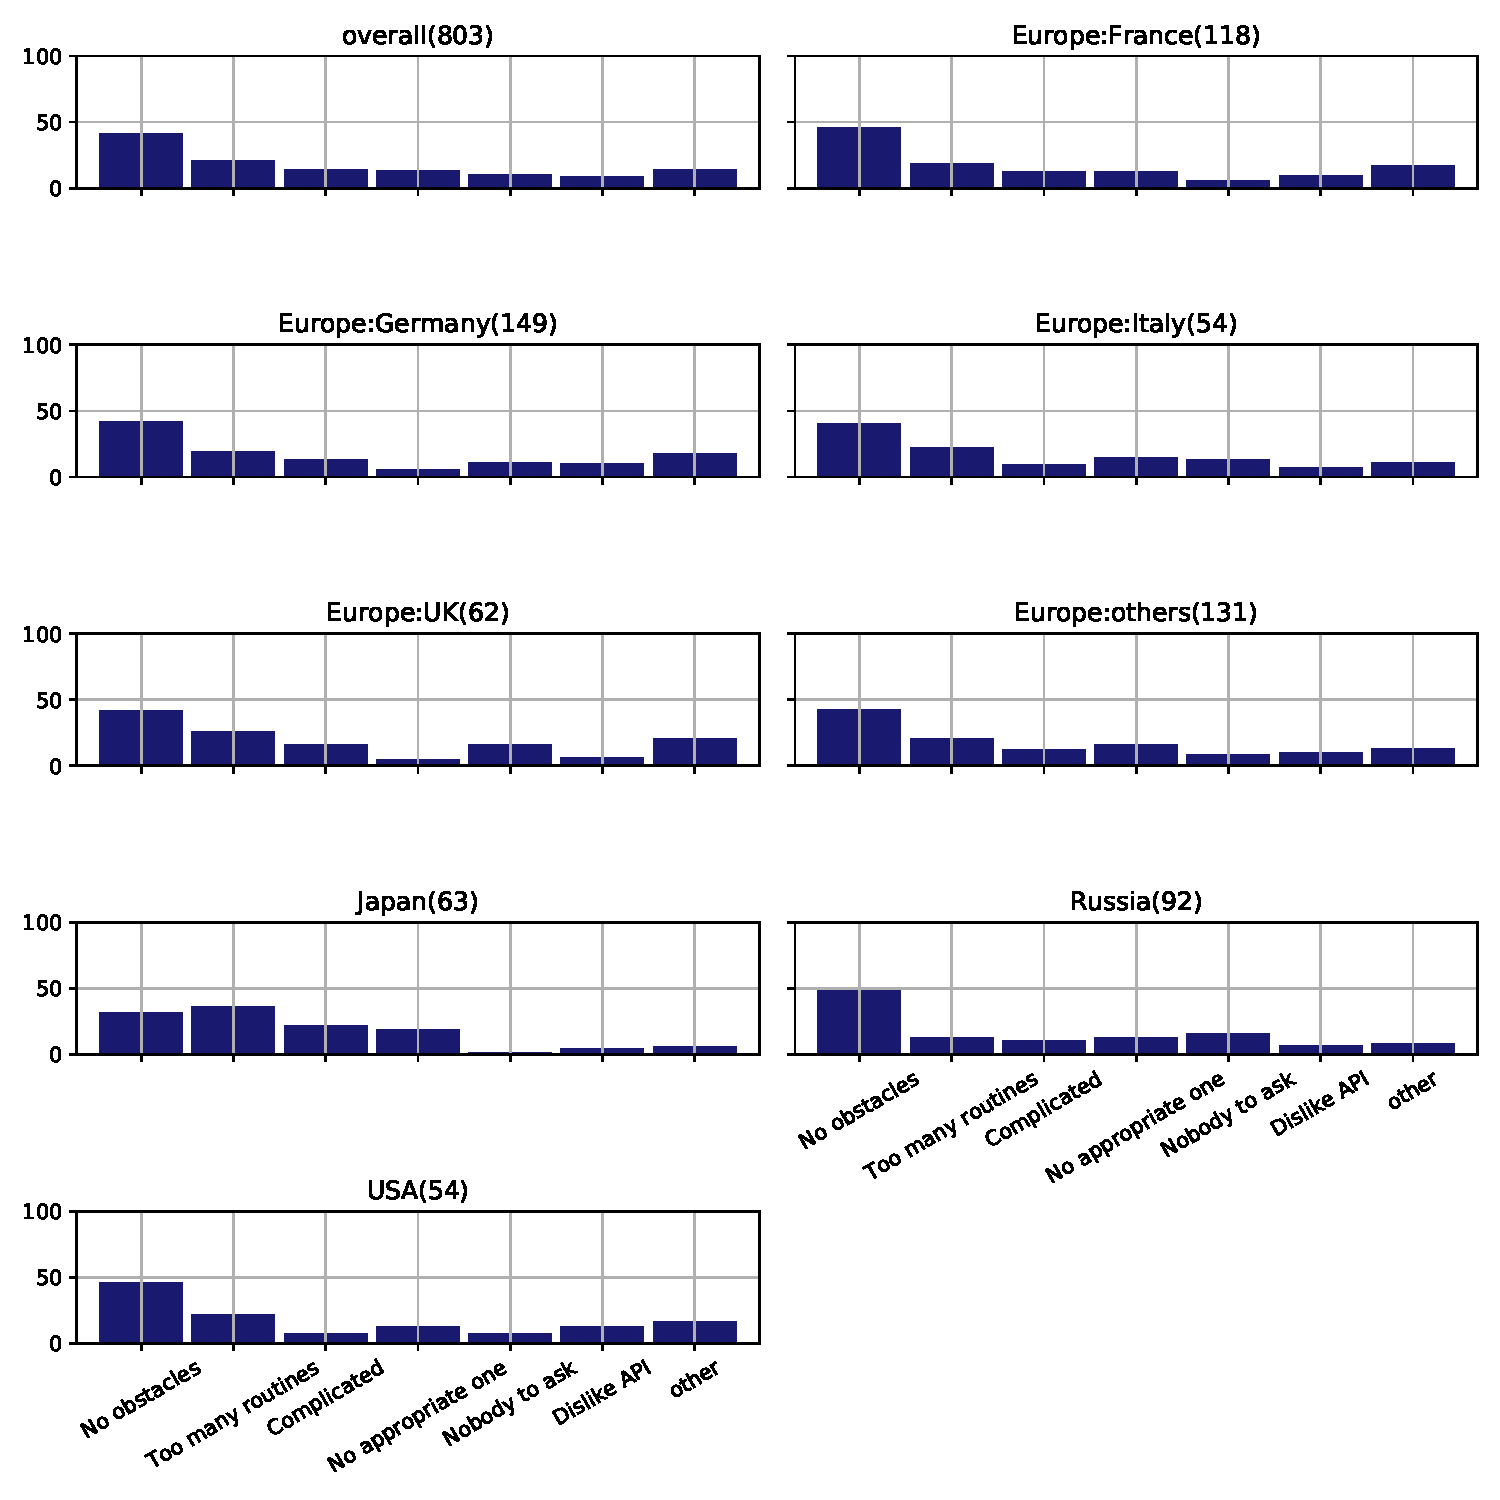
\includegraphics[width=10cm]{../pdfs/Q19.pdf}
\caption{Simple analysis: Q19}
\label{fig:Q19}
\end{center}
\end{figure}

\begin{figure}[htb]
\begin{center}
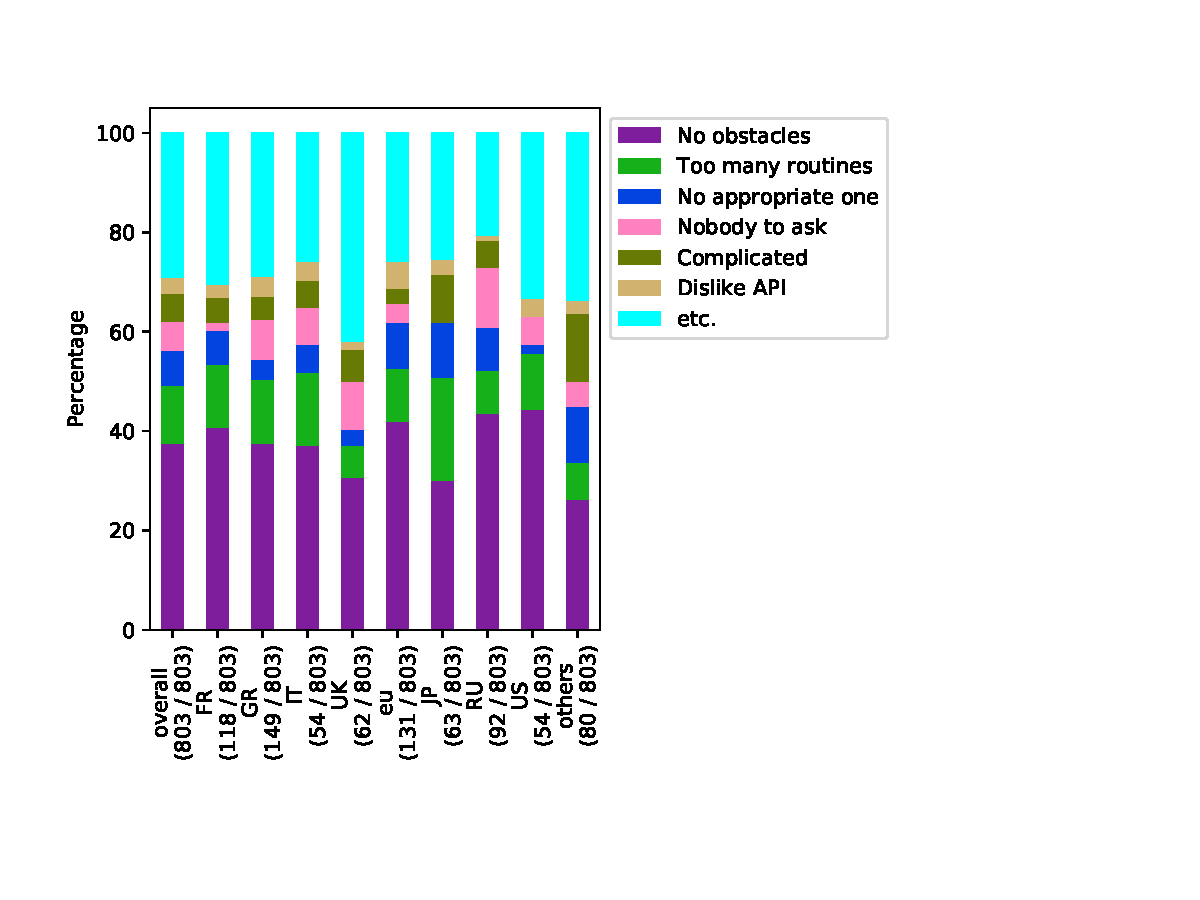
\includegraphics[width=14cm]{../pdfs/Q19-mans.pdf}
\caption{Multiple Answers: Q19}
\label{fig:Q19-mans}
\end{center}
\end{figure}

Many Japanese think the MPI standard provides too many routines, whereas the
answer of having no obstacles dominates in the other countries. In UK and
Germany, the percentage of answer having no appropriate lecture (book nor
tutorial) are relatively small. In UK, however, the percentage of answer having
nobody to ask is large as well as the one of Russia. This situation UK is very
interesting.
